\documentclass{standalone}

\usepackage{amsmath}
\usepackage{hyperref}
\usepackage{tikz}
\usepackage{graphicx}

\usetikzlibrary{decorations.pathreplacing,
  arrows,
  calc,
  decorations.pathmorphing,
  decorations.pathreplacing,
  decorations.markings,
  fadings,
  positioning,
  shapes,
  arrows.meta
}
\tikzstyle{snakearrow} = [decorate, decoration={pre length=0.1cm,
  post length=0.1cm, snake, amplitude=.4mm,
  segment length=4mm},thick, ->]
\usepgfmodule{oo}

\pgfdeclareradialshading{glow2}{\pgfpoint{0cm}{0cm}}{
  color(0mm)=(white);
  color(2mm)=(white);
  color(8mm)=(black);
  color(10mm)=(black)
}
\pgfdeclareradialshading{glow}{\pgfpoint{0cm}{0cm}}{
  color(0mm)=(white);
  color(5mm)=(white);
  color(9mm)=(black);
  color(10mm)=(black)
}

\begin{tikzfadingfrompicture}[name=glow fading]
  \shade [shading=glow] (0,0) circle (1);
\end{tikzfadingfrompicture}

\begin{tikzfadingfrompicture}[name=glow2 fading]
  \shade [shading=glow2] (0,0) circle (1);
\end{tikzfadingfrompicture}

\definecolor{atomorange}{rgb}{1.0,0.483,0.0}
\definecolor{pyplotc0}{rgb}{0.122,0.467,0.706}
\definecolor{pyplotc1}{rgb}{1.000,0.498,0.055}
\definecolor{pyplotc2}{rgb}{0.173,0.627,0.173}
\definecolor{pyplotc3}{rgb}{0.839,0.153,0.157}
\definecolor{pyplotc4}{rgb}{0.580,0.404,0.741}
\definecolor{pyplotc5}{rgb}{0.549,0.337,0.294}
\definecolor{pyplotc6}{rgb}{0.890,0.467,0.761}
\definecolor{pyplotc7}{rgb}{0.498,0.498,0.498}
\definecolor{pyplotc8}{rgb}{0.737,0.741,0.133}
\definecolor{pyplotc9}{rgb}{0.090,0.745,0.812}

\pgfdeclarelayer{tweezer}
\pgfsetlayers{tweezer,main}
\pgfooclass{tweezer}{
  \method tweezer() {
  }
  \method drawTweezer(#1,#2,#3) {
    \shade[shading=radial,path fading=glow fading,shift={(#1,#2)},rotate=90,yscale=1,
    fill opacity=0.9,inner color=#3]
    plot[draw,samples=200,domain=-4.5:4.5] function {sqrt(0.02 + (x)**2 / 10)}
    -- plot[draw,samples=200,domain=4.5:-4.5] function {-sqrt(0.02 + (x)**2 / 10)};
  }
  \method drawRaman(#1,#2) {
    \pgfoothis.drawTweezer(#1,#2,pyplotc4);
  }
  \method drawAtom(#1,#2,#3,#4) {
    \fill [#4,path fading=glow2 fading] (#1,#2) circle (#3);
  }
  \method drawDownAtom(#1,#2,#3) {
    \pgfoothis.drawAtom(#1,#2,#3,pyplotc0);
  }
  \method drawUpAtom(#1,#2,#3) {
    \pgfoothis.drawAtom(#1,#2,#3,pyplotc1);
  }
}
\pgfoonew \mytweezer=new tweezer()

\ifpdf
  % Ensure reproducible output
  \pdfinfoomitdate=1
  \pdfsuppressptexinfo=-1
  \pdftrailerid{}
  \hypersetup{
    pdfcreator={},
    pdfproducer={}
  }
\fi

\begin{document}
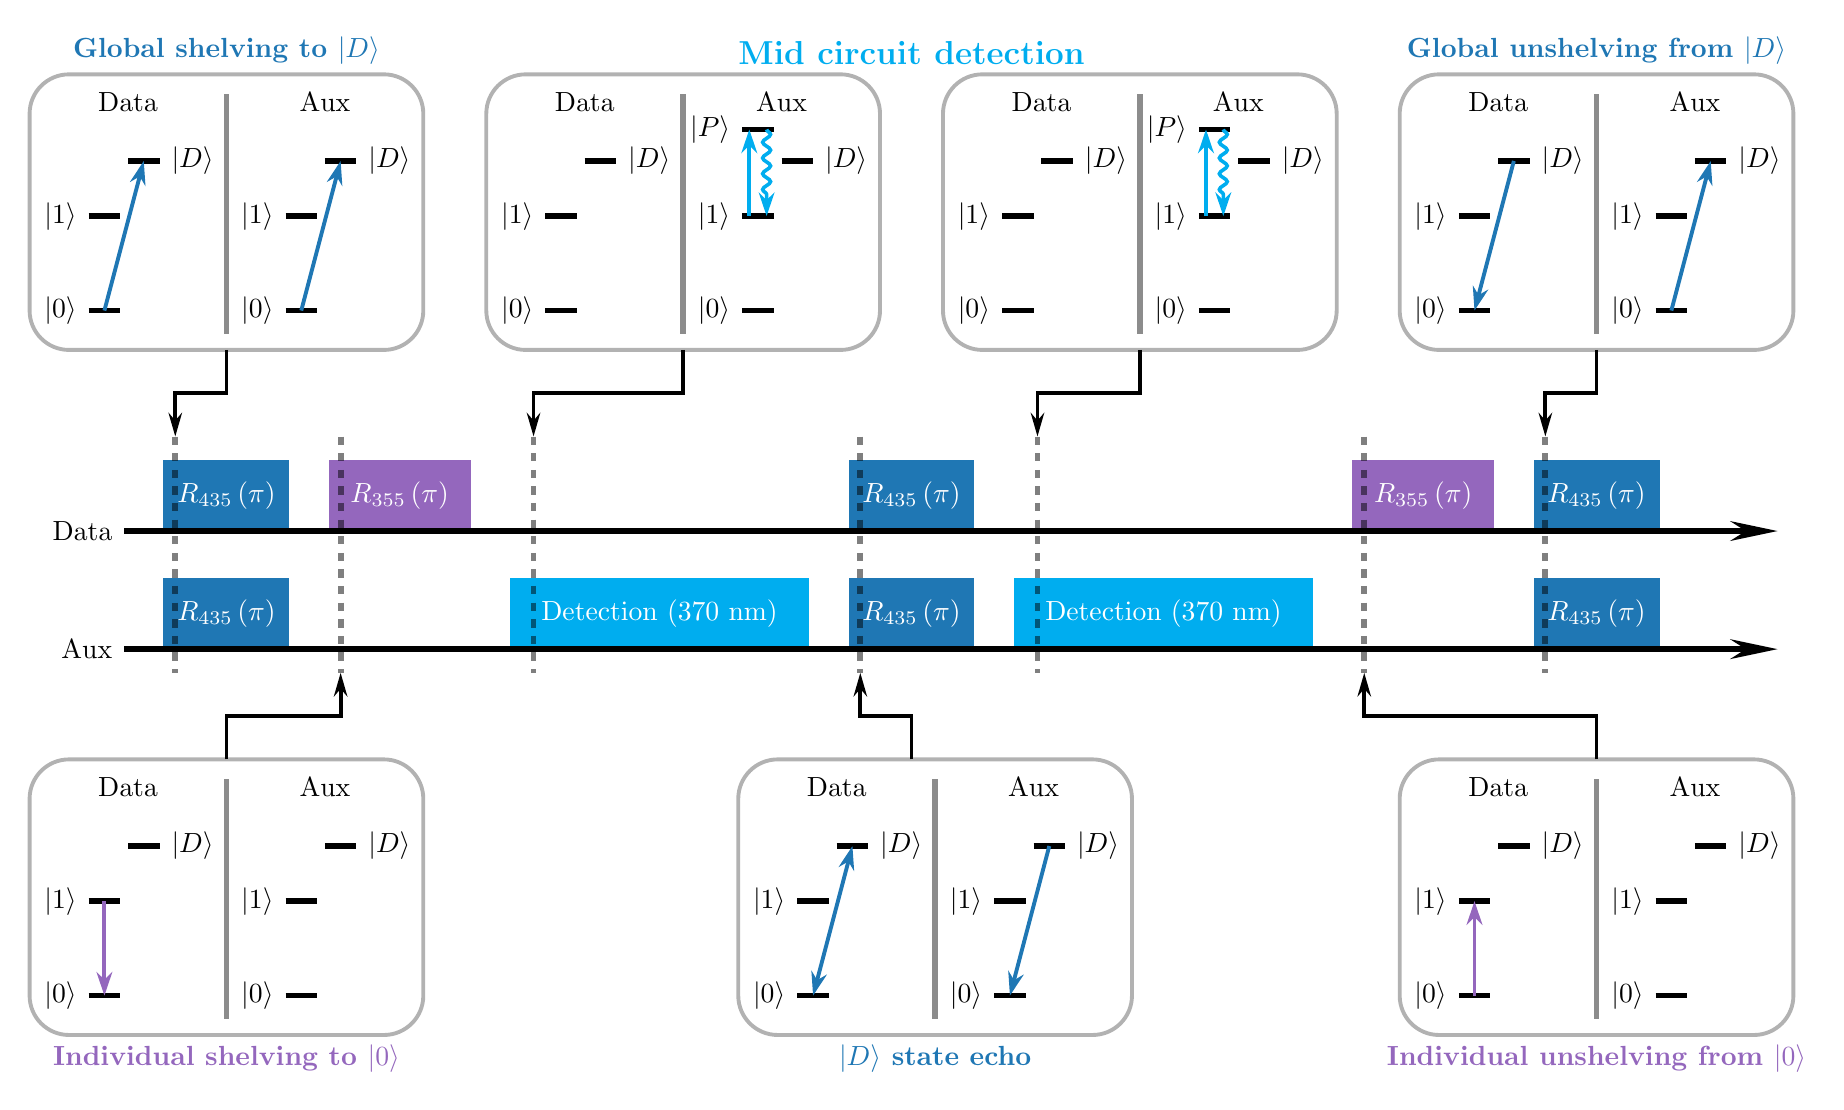
\begin{tikzpicture}
  \begin{scope}
    \fill[color=pyplotc0] (-9.5, 0) rectangle (-7.9, 0.9)
    node[white,pos=.5,align=center] {$R_{435}\left(\pi\right)$};
    \fill[color=pyplotc4] (-7.4, 0) rectangle (-5.6, 0.9)
    node[white,pos=.5] {$R_{355}\left(\pi\right)$};
    \fill[color=pyplotc0] (-0.8, 0) rectangle (0.8, 0.9)
    node[white,pos=.5,align=center] {$R_{435}\left(\pi\right)$};
    \fill[color=pyplotc4] (5.6, 0) rectangle (7.4, 0.9)
    node[white,pos=.5] {$R_{355}\left(\pi\right)$};
    \fill[color=pyplotc0] (7.9, 0) rectangle (9.5, 0.9)
    node[white,pos=.5,align=center] {$R_{435}\left(\pi\right)$};
    \draw[-{Stealth[length=6mm,width=2.5mm]},line width=2]
    (-10, 0) node[left] {Data} -- (11, 0);
  \end{scope}

  \begin{scope}[shift={(0, -1.5)}]
    \fill[color=pyplotc0] (-9.5, 0) rectangle (-7.9, 0.9)
    node[white,pos=.5,align=center] {$R_{435}\left(\pi\right)$};
    \fill[color=cyan] (-5.1, 0) rectangle (-1.3, 0.9)
    node[white,pos=.5,align=center] {Detection ($370$ nm)};
    \fill[color=pyplotc0] (-0.8, 0) rectangle (0.8, 0.9)
    node[white,pos=.5,align=center] {$R_{435}\left(\pi\right)$};
    \fill[color=cyan] (1.3, 0) rectangle (5.1, 0.9)
    node[white,pos=.5,align=center] {Detection ($370$ nm)};
    \fill[color=pyplotc0] (7.9, 0) rectangle (9.5, 0.9)
    node[white,pos=.5,align=center] {$R_{435}\left(\pi\right)$};
    \draw[-{Stealth[length=6mm,width=2.5mm]},line width=2]
    (-10, 0) node[left] {Aux} -- (11, 0);
  \end{scope}

  \begin{scope}[shift={(-9, 4)}]
    \begin{scope}[shift={(-1.25, 0)}]
      \node[above] at (0.3, 1.2) {Data};
      \draw[line width=2] (-0.2, 0) node[left] {$|1\rangle$} -- (0.2, 0);
      \draw[line width=2] (-0.2, -1.2) node[left] {$|0\rangle$} -- (0.2, -1.2);
      \draw[line width=2] (0.3, 0.7) -- (0.7, 0.7) node[right] {$|D\rangle$};

      \draw[pyplotc0,-{Stealth[length=3mm,width=2mm]},line width=1.4]
      (0, -1.2) -- (0.5, 0.7);

      \mytweezer.drawUpAtom(0, 0, 0.17)
      \mytweezer.drawDownAtom(0, -1.2, 0.17)
    \end{scope}

    \begin{scope}[shift={(1.25, 0)}]
      \node[above] at (0.3, 1.2) {Aux};
      \draw[line width=2] (-0.2, 0) node[left] {$|1\rangle$} -- (0.2, 0);
      \draw[line width=2] (-0.2, -1.2) node[left] {$|0\rangle$} -- (0.2, -1.2);
      \draw[line width=2] (0.3, 0.7) -- (0.7, 0.7) node[right] {$|D\rangle$};

      \draw[pyplotc0,-{Stealth[length=3mm,width=2mm]},line width=1.4]
      (0, -1.2) -- (0.5, 0.7);

      \mytweezer.drawUpAtom(0, 0, 0.17)
      \mytweezer.drawDownAtom(0, -1.2, 0.17)
    \end{scope}
    \draw[line width=2,opacity=0.45] (0.3, 1.55) -- (0.3, -1.5);
    \draw[rounded corners=0.5cm, line width=1.4, opacity=0.3]
    (-2.2, -1.7) rectangle (2.8, 1.8);
    \node[color=pyplotc0, above] at (0.3, 1.8)
    {\textbf{Global shelving to $|D\rangle$}};
  \end{scope}

  \draw[dashed, line width=2.1, opacity=0.5] (-9.35, 1.2) -- (-9.35, -1.8);
  \draw[-{Stealth[length=3mm,width=1.7mm]},line width=1.4]
  (-8.7, 2.3) -- (-8.7, 1.75) -| (-9.35, 1.2);

  \begin{scope}[shift={(-9, -4.7)}]
    \begin{scope}[shift={(-1.25, 0)}]
      \node[above] at (0.3, 1.2) {Data};
      \draw[line width=2] (-0.2, 0) node[left] {$|1\rangle$} -- (0.2, 0);
      \draw[line width=2] (-0.2, -1.2) node[left] {$|0\rangle$} -- (0.2, -1.2);
      \draw[line width=2] (0.3, 0.7) -- (0.7, 0.7) node[right] {$|D\rangle$};

      \draw[pyplotc4,-{Stealth[length=3mm,width=2mm]},line width=1.4]
      (0, 0) -- (0, -1.2);

      \mytweezer.drawUpAtom(0, 0, 0.17)
      \mytweezer.drawDownAtom(0.5, 0.7, 0.17)
    \end{scope}

    \begin{scope}[shift={(1.25, 0)}]
      \node[above] at (0.3, 1.2) {Aux};
      \draw[line width=2] (-0.2, 0) node[left] {$|1\rangle$} -- (0.2, 0);
      \draw[line width=2] (-0.2, -1.2) node[left] {$|0\rangle$} -- (0.2, -1.2);
      \draw[line width=2] (0.3, 0.7) -- (0.7, 0.7) node[right] {$|D\rangle$};

      \mytweezer.drawUpAtom(0, 0, 0.17)
      \mytweezer.drawDownAtom(0.5, 0.7, 0.17)
    \end{scope}
    \draw[line width=2,opacity=0.45] (0.3, 1.55) -- (0.3, -1.5);
    \draw[rounded corners=0.5cm, line width=1.4, opacity=0.3]
    (-2.2, -1.7) rectangle (2.8, 1.8);
    \node[color=pyplotc4, below] at (0.3, -1.7)
    {\textbf{Individual shelving to $|0\rangle$}};
  \end{scope}

  \draw[dashed, line width=2.1, opacity=0.5] (-7.25, 1.2) -- (-7.25, -1.8);
  \draw[-{Stealth[length=3mm,width=1.7mm]},line width=1.4]
  (-8.7, -2.9) -- (-8.7, -2.35) -| (-7.25, -1.8);

  \begin{scope}[shift={(-3.2, 4)}]
    \begin{scope}[shift={(-1.25, 0)}]
      \node[above] at (0.3, 1.2) {Data};
      \draw[line width=2] (-0.2, 0) node[left] {$|1\rangle$} -- (0.2, 0);
      \draw[line width=2] (-0.2, -1.2) node[left] {$|0\rangle$} -- (0.2, -1.2);
      \draw[line width=2] (0.3, 0.7) -- (0.7, 0.7) node[right] {$|D\rangle$};

      \mytweezer.drawUpAtom(0, -1.2, 0.17)
      \mytweezer.drawDownAtom(0.5, 0.7, 0.17)
    \end{scope}

    \begin{scope}[shift={(1.25, 0)}]
      \node[above] at (0.3, 1.2) {Aux};
      \draw[line width=2] (-0.2, 1.1) node[left] {$|P\rangle$} -- (0.2, 1.1);
      \draw[line width=2] (-0.2, 0) node[left] {$|1\rangle$} -- (0.2, 0);
      \draw[line width=2] (-0.2, -1.2) node[left] {$|0\rangle$} -- (0.2, -1.2);
      \draw[line width=2] (0.3, 0.7) -- (0.7, 0.7) node[right] {$|D\rangle$};

      \draw[cyan,-{Stealth[length=3mm,width=2mm]},line width=1.4]
      (-0.11, 0) -- (-0.11, 1.1);
      \draw[cyan,-{Stealth[length=3mm,width=2mm]},line width=1.3,
      decorate, decoration={pre length=0cm,
        post length=2mm, snake, amplitude=0.5mm,
        segment length=2mm}] (0.11, 1.1) -- (0.11, 0);

      \mytweezer.drawUpAtom(0, 0, 0.17)
      \mytweezer.drawDownAtom(0.5, 0.7, 0.17)
    \end{scope}
    \draw[line width=2,opacity=0.45] (0.3, 1.55) -- (0.3, -1.5);
    \draw[rounded corners=0.5cm, line width=1.4, opacity=0.3]
    (-2.2, -1.7) rectangle (2.8, 1.8);
  \end{scope}

  \draw[dashed, line width=2.1, opacity=0.5] (-4.8, 1.2) -- (-4.8, -1.8);
  \draw[-{Stealth[length=3mm,width=1.7mm]},line width=1.4]
  (-2.9, 2.3) -- (-2.9, 1.75) -| (-4.8, 1.2);

  \begin{scope}[shift={(2.6, 4)}]
    \begin{scope}[shift={(-1.25, 0)}]
      \node[above] at (0.3, 1.2) {Data};
      \draw[line width=2] (-0.2, 0) node[left] {$|1\rangle$} -- (0.2, 0);
      \draw[line width=2] (-0.2, -1.2) node[left] {$|0\rangle$} -- (0.2, -1.2);
      \draw[line width=2] (0.3, 0.7) -- (0.7, 0.7) node[right] {$|D\rangle$};

      \mytweezer.drawUpAtom(0.5, 0.7, 0.17)
      \mytweezer.drawDownAtom(0, -1.2, 0.17)
    \end{scope}

    \begin{scope}[shift={(1.25, 0)}]
      \node[above] at (0.3, 1.2) {Aux};
      \draw[line width=2] (-0.2, 1.1) node[left] {$|P\rangle$} -- (0.2, 1.1);
      \draw[line width=2] (-0.2, 0) node[left] {$|1\rangle$} -- (0.2, 0);
      \draw[line width=2] (-0.2, -1.2) node[left] {$|0\rangle$} -- (0.2, -1.2);
      \draw[line width=2] (0.3, 0.7) -- (0.7, 0.7) node[right] {$|D\rangle$};

      \draw[cyan,-{Stealth[length=3mm,width=2mm]},line width=1.4]
      (-0.11, 0) -- (-0.11, 1.1);
      \draw[cyan,-{Stealth[length=3mm,width=2mm]},line width=1.3,
      decorate, decoration={pre length=0cm,
        post length=2mm, snake, amplitude=0.5mm,
        segment length=2mm}] (0.11, 1.1) -- (0.11, 0);

      \mytweezer.drawUpAtom(0, 0, 0.17)
      \mytweezer.drawDownAtom(0, -1.2, 0.17)
    \end{scope}
    \draw[line width=2,opacity=0.45] (0.3, 1.55) -- (0.3, -1.5);
    \draw[rounded corners=0.5cm, line width=1.4, opacity=0.3]
    (-2.2, -1.7) rectangle (2.8, 1.8);
  \end{scope}

  \draw[dashed, line width=2.1, opacity=0.5] (1.6, 1.2) -- (1.6, -1.8);
  \draw[-{Stealth[length=3mm,width=1.7mm]},line width=1.4]
  (2.9, 2.3) -- (2.9, 1.75) -| (1.6, 1.2);

  \node[color=cyan, above] at (0, 5.8)
    {\textbf{\large Mid circuit detection}};

  \begin{scope}[shift={(0, -4.7)}]
    \begin{scope}[shift={(-1.25, 0)}]
      \node[above] at (0.3, 1.2) {Data};
      \draw[line width=2] (-0.2, 0) node[left] {$|1\rangle$} -- (0.2, 0);
      \draw[line width=2] (-0.2, -1.2) node[left] {$|0\rangle$} -- (0.2, -1.2);
      \draw[line width=2] (0.3, 0.7) -- (0.7, 0.7) node[right] {$|D\rangle$};

      \draw[pyplotc0,{Stealth[length=3mm,width=2mm]}-{Stealth[length=3mm,width=2mm]},line width=1.4]
      (0, -1.2) -- (0.5, 0.7);

      \mytweezer.drawUpAtom(0, -1.2, 0.17)
      \mytweezer.drawDownAtom(0.5, 0.7, 0.17)
    \end{scope}

    \begin{scope}[shift={(1.25, 0)}]
      \node[above] at (0.3, 1.2) {Aux};
      \draw[line width=2] (-0.2, 0) node[left] {$|1\rangle$} -- (0.2, 0);
      \draw[line width=2] (-0.2, -1.2) node[left] {$|0\rangle$} -- (0.2, -1.2);
      \draw[line width=2] (0.3, 0.7) -- (0.7, 0.7) node[right] {$|D\rangle$};

      \draw[pyplotc0,-{Stealth[length=3mm,width=2mm]},line width=1.4]
      (0.5, 0.7) -- (0, -1.2);

      \mytweezer.drawUpAtom(0, 0, 0.17)
      \mytweezer.drawDownAtom(0.5, 0.7, 0.17)
    \end{scope}
    \draw[line width=2,opacity=0.45] (0.3, 1.55) -- (0.3, -1.5);
    \draw[rounded corners=0.5cm, line width=1.4, opacity=0.3]
    (-2.2, -1.7) rectangle (2.8, 1.8);
    \node[color=pyplotc0, below] at (0.3, -1.7)
    {\textbf{$|D\rangle$ state echo}};
  \end{scope}

  \draw[dashed, line width=2.1, opacity=0.5] (-0.65, 1.2) -- (-0.65, -1.8);
  \draw[-{Stealth[length=3mm,width=1.7mm]},line width=1.4]
  (0, -2.9) -- (0, -2.35) -| (-0.65, -1.8);

  \begin{scope}[shift={(8.4, -4.7)}]
    \begin{scope}[shift={(-1.25, 0)}]
      \node[above] at (0.3, 1.2) {Data};
      \draw[line width=2] (-0.2, 0) node[left] {$|1\rangle$} -- (0.2, 0);
      \draw[line width=2] (-0.2, -1.2) node[left] {$|0\rangle$} -- (0.2, -1.2);
      \draw[line width=2] (0.3, 0.7) -- (0.7, 0.7) node[right] {$|D\rangle$};

      \draw[pyplotc4,-{Stealth[length=3mm,width=2mm]},line width=1.4]
      (0, -1.2) -- (0, 0);

      \mytweezer.drawUpAtom(0.5, 0.7, 0.17)
      \mytweezer.drawDownAtom(0, -1.2, 0.17)
    \end{scope}

    \begin{scope}[shift={(1.25, 0)}]
      \node[above] at (0.3, 1.2) {Aux};
      \draw[line width=2] (-0.2, 0) node[left] {$|1\rangle$} -- (0.2, 0);
      \draw[line width=2] (-0.2, -1.2) node[left] {$|0\rangle$} -- (0.2, -1.2);
      \draw[line width=2] (0.3, 0.7) -- (0.7, 0.7) node[right] {$|D\rangle$};

      \mytweezer.drawUpAtom(0, 0, 0.17)
      \mytweezer.drawDownAtom(0, -1.2, 0.17)
    \end{scope}
    \draw[line width=2,opacity=0.45] (0.3, 1.55) -- (0.3, -1.5);
    \draw[rounded corners=0.5cm, line width=1.4, opacity=0.3]
    (-2.2, -1.7) rectangle (2.8, 1.8);
    \node[color=pyplotc4, below] at (0.3, -1.7)
    {\textbf{Individual unshelving from $|0\rangle$}};
  \end{scope}

  \draw[dashed, line width=2.1, opacity=0.5] (5.75, 1.2) -- (5.75, -1.8);
  \draw[-{Stealth[length=3mm,width=1.7mm]},line width=1.4]
  (8.7, -2.9) -- (8.7, -2.35) -| (5.75, -1.8);

  \begin{scope}[shift={(8.4, 4)}]
    \begin{scope}[shift={(-1.25, 0)}]
      \node[above] at (0.3, 1.2) {Data};
      \draw[line width=2] (-0.2, 0) node[left] {$|1\rangle$} -- (0.2, 0);
      \draw[line width=2] (-0.2, -1.2) node[left] {$|0\rangle$} -- (0.2, -1.2);
      \draw[line width=2] (0.3, 0.7) -- (0.7, 0.7) node[right] {$|D\rangle$};

      \draw[pyplotc0,-{Stealth[length=3mm,width=2mm]},line width=1.4]
      (0.5, 0.7) -- (0, -1.2);

      \mytweezer.drawUpAtom(0.5, 0.7, 0.17)
      \mytweezer.drawDownAtom(0, 0, 0.17)
    \end{scope}

    \begin{scope}[shift={(1.25, 0)}]
      \node[above] at (0.3, 1.2) {Aux};
      \draw[line width=2] (-0.2, 0) node[left] {$|1\rangle$} -- (0.2, 0);
      \draw[line width=2] (-0.2, -1.2) node[left] {$|0\rangle$} -- (0.2, -1.2);
      \draw[line width=2] (0.3, 0.7) -- (0.7, 0.7) node[right] {$|D\rangle$};

      \draw[pyplotc0,-{Stealth[length=3mm,width=2mm]},line width=1.4]
      (0, -1.2) -- (0.5, 0.7);

      \mytweezer.drawUpAtom(0, 0, 0.17)
      \mytweezer.drawDownAtom(0, -1.2, 0.17)
    \end{scope}
    \draw[line width=2,opacity=0.45] (0.3, 1.55) -- (0.3, -1.5);
    \draw[rounded corners=0.5cm, line width=1.4, opacity=0.3]
    (-2.2, -1.7) rectangle (2.8, 1.8);
    \node[color=pyplotc0, above] at (0.3, 1.8)
    {\textbf{Global unshelving from $|D\rangle$}};
  \end{scope}

  \draw[dashed, line width=2.1, opacity=0.5] (8.05, 1.2) -- (8.05, -1.8);
  \draw[-{Stealth[length=3mm,width=1.7mm]},line width=1.4]
  (8.7, 2.3) -- (8.7, 1.75) -| (8.05, 1.2);
\end{tikzpicture}
\end{document}
